% ============================================================
\chapter{Data Manipulation with Pandas}
\label{ch:pandas}
% ============================================================

\section{Introduction to Pandas}

\textbf{Pandas}\index{Pandas} is the central library for data science in Python. It provides two fundamental data structures: the \py{Series} (indexed vector) and the \py{DataFrame} (indexed table).

\begin{definition}[DataFrame]
A \textbf{DataFrame} is a two-dimensional table with labels for rows (index) and columns. Each column is a \py{Series} of the same length.
\end{definition}

\section{Creating DataFrames}

\begin{codeblock}[title=\textbf{Python --- Creation}]
\begin{minted}{python}
import pandas as pd
import numpy as np

# From a dictionary
data = {
    'Name': ['Alice', 'Bob', 'Charlie', 'Diana'],
    'Age': [25, 30, 35, 28],
    'Salary': [45000, 55000, 70000, 52000],
    'City': ['Paris', 'Lyon', 'Paris', 'Marseille']
}
df = pd.DataFrame(data)
print(df)
print(f"\nShape: {df.shape}")
print(f"Types:\n{df.dtypes}")
\end{minted}
\end{codeblock}

\begin{codeoutput}
\begin{verbatim}
       Name  Age  Salary      City
0    Alice   25    45000      Paris
1      Bob   30    55000       Lyon
2  Charlie   35    70000      Paris
3    Diana   28    52000  Marseille

Shape: (4, 4)
Types:
Name      object
Age        int64
Salary     int64
City      object
dtype: object
\end{verbatim}
\end{codeoutput}

\section{Loading Data}

\begin{codeblock}[title=\textbf{Python --- Reading files}]
\begin{minted}{python}
# CSV (most common)
# df = pd.read_csv('data.csv')
# df = pd.read_csv('data.csv', sep=';', encoding='utf-8')

# From Seaborn (built-in datasets)
import seaborn as sns
tips = sns.load_dataset('tips')   # restaurant tips
print(f"Shape: {tips.shape}")
print(tips.head(3))
\end{minted}
\end{codeblock}

\begin{codeoutput}
\begin{verbatim}
Shape: (244, 7)
   total_bill   tip     sex smoker  day    time  size
0       16.99  1.01  Female     No  Sun  Dinner     2
1       10.34  1.66    Male     No  Sun  Dinner     3
2       21.01  3.50    Male     No  Sun  Dinner     3
\end{verbatim}
\end{codeoutput}

\section{Selection and Indexing}

\begin{keyformulas}[title=\textbf{Selection Methods}]
\begin{tabular}{ll}
\toprule
\textbf{Syntax} & \textbf{Description} \\
\midrule
\py{df['col']} & Select one column (Series) \\
\py{df[['c1','c2']]} & Select multiple columns \\
\py{df.loc[i, 'col']} & Select by label \\
\py{df.iloc[i, j]} & Select by position \\
\py{df[df['col'] > x]} & Boolean filtering \\
\bottomrule
\end{tabular}
\end{keyformulas}

\begin{codeblock}[title=\textbf{Python --- Selection}]
\begin{minted}{python}
import seaborn as sns
tips = sns.load_dataset('tips')

# Column selection
print("--- Single column ---")
print(tips['total_bill'].head(3))

# Filtering
big_tips = tips[tips['tip'] > 5]
print(f"\n--- Tips > $5: {len(big_tips)} rows ---")
print(big_tips.head(3))

# Combined selection
print("\n--- loc: females, Sunday ---")
mask = (tips['sex'] == 'Female') & (tips['day'] == 'Sun')
print(tips.loc[mask, ['total_bill', 'tip']].head(3))
\end{minted}
\end{codeblock}

\begin{codeoutput}
\begin{verbatim}
--- Single column ---
0    16.99
1    10.34
2    21.01
Name: total_bill, dtype: float64

--- Tips > $5: 17 rows ---
     total_bill   tip   sex smoker  day    time  size
23        39.42  7.58  Male     No  Sat  Dinner     4
44        30.40  5.60  Male     No  Sun  Dinner     4
47        32.40  6.00  Male     No  Sun  Dinner     4

--- loc: females, Sunday ---
     total_bill   tip
0         16.99  1.01
5         25.29  4.71
15        21.58  3.92
\end{verbatim}
\end{codeoutput}

\section{Modifying and Adding Columns}

\begin{codeblock}[title=\textbf{Python --- New columns}]
\begin{minted}{python}
# Add a computed column
tips['tip_pct'] = (tips['tip'] / tips['total_bill'] * 100).round(1)
print(tips[['total_bill', 'tip', 'tip_pct']].head(5))

# Apply a function
tips['bill_category'] = tips['total_bill'].apply(
    lambda x: 'High' if x > 30 else ('Medium' if x > 15 else 'Low'))
print(tips['bill_category'].value_counts())
\end{minted}
\end{codeblock}

\begin{codeoutput}
\begin{verbatim}
   total_bill   tip  tip_pct
0       16.99  1.01      5.9
1       10.34  1.66     16.1
2       21.01  3.50     16.7
3       23.68  3.31     14.0
4       24.59  3.61     14.7

bill_category
Medium    111
Low        69
High       64
Name: count, dtype: int64
\end{verbatim}
\end{codeoutput}

\section{Aggregation with \texttt{groupby}}

\begin{definition}[Split-Apply-Combine]\index{groupby}
The \textbf{split-apply-combine} paradigm consists of:
\begin{enumerate}
\item \textbf{Split}: divide data into groups.
\item \textbf{Apply}: apply a function (sum, mean, count\ldots) to each group.
\item \textbf{Combine}: assemble the results.
\end{enumerate}
\end{definition}

\begin{center}
\begin{tikzpicture}[
  block/.style={rectangle, draw, fill=#1!15, rounded corners,
    minimum width=2.2cm, minimum height=0.8cm, align=center, font=\small},
  arr/.style={-{Stealth}, thick}
]
\node[block=blue] (data) at (0,0) {Data};
\node[block=red] (g1) at (4,1) {Group A};
\node[block=red] (g2) at (4,0) {Group B};
\node[block=red] (g3) at (4,-1) {Group C};
\node[block=green] (r1) at (8,1) {Result A};
\node[block=green] (r2) at (8,0) {Result B};
\node[block=green] (r3) at (8,-1) {Result C};
\node[block=purple] (out) at (12,0) {Final Table};
\draw[arr] (data) -- node[above,font=\scriptsize]{Split} (g1);
\draw[arr] (data) -- (g2);
\draw[arr] (data) -- (g3);
\draw[arr] (g1) -- node[above,font=\scriptsize]{Apply} (r1);
\draw[arr] (g2) -- (r2);
\draw[arr] (g3) -- (r3);
\draw[arr] (r1) -- node[above,font=\scriptsize]{Combine} (out);
\draw[arr] (r2) -- (out);
\draw[arr] (r3) -- (out);
\end{tikzpicture}
\end{center}

\begin{codeblock}[title=\textbf{Python --- groupby}]
\begin{minted}{python}
# Mean by day
print("--- Mean by day ---")
print(tips.groupby('day')[['total_bill', 'tip']].mean().round(2))

# Multiple aggregations
print("\n--- Multiple aggregations ---")
agg = tips.groupby(['day', 'time']).agg(
    n_meals=('total_bill', 'count'),
    avg_bill=('total_bill', 'mean'),
    avg_tip=('tip', 'mean')
).round(2)
print(agg)
\end{minted}
\end{codeblock}

\begin{codeoutput}
\begin{verbatim}
--- Mean by day ---
      total_bill   tip
day
Thur       17.68  2.77
Fri        17.15  2.73
Sat        20.44  2.99
Sun        21.41  3.26

--- Multiple aggregations ---
             n_meals  avg_bill  avg_tip
day  time
Thur Lunch        61     17.66     2.77
     Dinner        1     18.78     3.00
Fri  Lunch         7     12.85     2.38
     Dinner       12     19.66     2.94
Sat  Dinner       87     20.44     2.99
Sun  Dinner       76     21.41     3.26
\end{verbatim}
\end{codeoutput}

\section{Pivot Tables}

\begin{codeblock}[title=\textbf{Python --- pivot\_table}]
\begin{minted}{python}
pivot = tips.pivot_table(
    values='tip', index='day', columns='sex',
    aggfunc='mean').round(2)
print(pivot)
\end{minted}
\end{codeblock}

\begin{codeoutput}
\begin{verbatim}
sex   Female  Male
day
Thur    2.58  2.88
Fri     2.78  2.69
Sat     2.80  3.08
Sun     3.37  3.22
\end{verbatim}
\end{codeoutput}

\section{Joins}

\begin{codeblock}[title=\textbf{Python --- merge}]
\begin{minted}{python}
# Two DataFrames
clients = pd.DataFrame({
    'client_id': [1, 2, 3, 4],
    'name': ['Alice', 'Bob', 'Charlie', 'Diana']
})
orders = pd.DataFrame({
    'order_id': [101, 102, 103, 104],
    'client_id': [1, 2, 2, 5],
    'amount': [150, 200, 80, 300]
})

# Inner join
inner = pd.merge(clients, orders, on='client_id', how='inner')
print("--- Inner join ---")
print(inner)

# Left join (keep all clients)
left = pd.merge(clients, orders, on='client_id', how='left')
print("\n--- Left join ---")
print(left)
\end{minted}
\end{codeblock}

\begin{codeoutput}
\begin{verbatim}
--- Inner join ---
   client_id     name  order_id  amount
0          1    Alice       101     150
1          2      Bob       102     200
2          2      Bob       103      80

--- Left join ---
   client_id     name  order_id  amount
0          1    Alice     101.0   150.0
1          2      Bob     102.0   200.0
2          2      Bob     103.0    80.0
3          3  Charlie       NaN     NaN
4          4    Diana       NaN     NaN
\end{verbatim}
\end{codeoutput}

\begin{center}
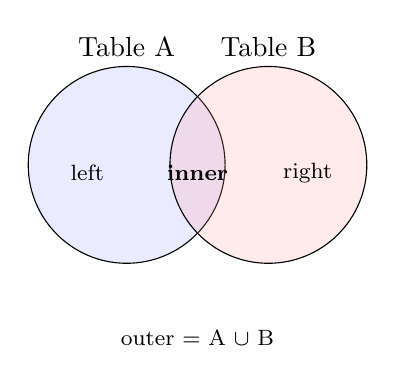
\begin{tikzpicture}[
  set/.style={circle, draw, minimum size=2.5cm, fill opacity=0.2, text opacity=1}
]
\node[set, fill=blue!40, label=above:{Table A}] (A) at (0,0) {};
\node[set, fill=red!40, label=above:{Table B}] (B) at (1.8,0) {};
\node at (0.9, -0.1) {\footnotesize\textbf{inner}};
\node at (-0.5, -0.1) {\footnotesize left};
\node at (2.3, -0.1) {\footnotesize right};
\node at (0.9, -2.2) {\footnotesize outer = A $\cup$ B};
\end{tikzpicture}
\end{center}

\section{Sorting and Ranking}

\begin{codeblock}[title=\textbf{Python --- Sorting}]
\begin{minted}{python}
# Sort by tip descending
top5 = tips.nlargest(5, 'tip')[['total_bill', 'tip', 'day']]
print(top5)

# Rank
tips['tip_rank'] = tips['tip'].rank(ascending=False).astype(int)
print(tips[['total_bill', 'tip', 'tip_rank']].head(5))
\end{minted}
\end{codeblock}

\begin{codeoutput}
\begin{verbatim}
     total_bill   tip  day
170       50.81 10.00  Sat
212       48.33  9.00  Sat
23        39.42  7.58  Sat
59        48.27  6.73  Sat
183       23.17  6.50  Sun

   total_bill   tip  tip_rank
0       16.99  1.01       224
1       10.34  1.66       188
2       21.01  3.50        52
3       23.68  3.31        63
4       24.59  3.61        46
\end{verbatim}
\end{codeoutput}

\section{String Operations}

\begin{codeblock}[title=\textbf{Python --- \texttt{.str} accessor}]
\begin{minted}{python}
names = pd.Series(['  Alice Dupont  ', 'bob martin', 'CHARLIE PETIT'])

print(names.str.strip().str.title())
print(names.str.contains('art', case=False))
\end{minted}
\end{codeblock}

\begin{codeoutput}
\begin{verbatim}
0     Alice Dupont
1       Bob Martin
2    Charlie Petit
dtype: object
0    False
1     True
2    False
dtype: bool
\end{verbatim}
\end{codeoutput}

\section{Exercises}

\begin{exercise}[$\star$]
Load the \py{tips} dataset from Seaborn. Display the number of meals by day of the week and by time (lunch/dinner).
\end{exercise}

\begin{exercise}[$\star$]
Create a DataFrame with 5 students, their math and physics grades. Add an ``average'' column and sort by descending average.
\end{exercise}

\begin{exercise}[$\star\star$]
On the Tips dataset, compute for each combination (sex, smoker): the number of meals, the average bill, and the average tip percentage.
\end{exercise}

\begin{exercise}[$\star\star$]
Create two DataFrames: one with products (id, name, category), one with sales (product\_id, quantity, date). Join them and compute revenue by category.
\end{exercise}

\begin{exercise}[$\star\star\star$]
Write a function that takes a DataFrame and returns an automatic report: number of rows, column types, percentage of missing values per column, number of duplicates.
\end{exercise}

\begin{keyformulas}[title=\textbf{Essential Pandas Functions}]
\begin{itemize}
\item \py{pd.read_csv()}, \py{df.to_csv()} --- import/export
\item \py{df.head()}, \py{df.info()}, \py{df.describe()} --- exploration
\item \py{df.loc[]}, \py{df.iloc[]} --- selection
\item \py{df.groupby().agg()} --- aggregation
\item \py{pd.merge()} --- joins
\item \py{df.sort_values()}, \py{df.nlargest()} --- sorting
\end{itemize}
\end{keyformulas}
